\newpage
\section{Distributed Shared Memory}
\label{sec:shared}


\noindent
To speed up computation on a single machine, we use multiple cores to 
run OS threads in parallel. Consider the following example:

\begin{lstlisting}[language=Go]
    for (i := 0; i< n; i++) {
        go work(i,results);
    }  
\end{lstlisting}

\noindent
Here our goal is to run some function \texttt{work} on a perhaps large 
data set of $n$ size. Go easily abstracts this away with the \texttt{go} keyword.\\

\noindent
Now, what if we want to run this on a distributed system?

\begin{lstlisting}[language=Go]
    package main
    import (
        "net/rpc"
    )
    type Args struct{}
    type WorkServer int64
    func (t *WorkServer) DoWork(args *Args, reply *int64) error {
        // Fill reply pointer to send the data back
        work(args.data, *reply);
        return nil
    }
\end{lstlisting}

\noindent
We have to decide now on a system of communication:
\begin{itemize}
    \item How do we interact with sending and receiving data (conflicts, failures, etc.)
    \item How should our coordinator dispatch the work?
    \item What RPCs should we include in our API?
\end{itemize}

\noindent
To solve this problem, we reuse a hardware primitive in the previous Section (\ref{sec:virt}).
\begin{theo}[Multithread Comminucation -- Virtual Memory]

    A multithread process can still communicate between threads by utilizing the same virtual memory space, we call this \textbf{shared memory}.
\end{theo}
\noindent
\underline{\textbf{The goal} is to bring this primitive to the distributed system level.}

\newpage 

\noindent
We clearly define our problem-space:

\begin{Def}[Distributed Shared Memory]
    
    A \textbf{Distributed Shared Memory (DSM)} system is a system that allows multiple processes on different machines to access a shared memory space as if it were local.
    I.e,. create the illusion of a single shared memory across multiple machines to enable multithreaded programs in a distrusted setting.\\

    \noindent
    Applications are built on top of a DSM system who abstracts away consensus and communication. DSM systems 
    connect to the underlying hardware support for shared memory (virtual address translation) to coordinate.
    Page faults are redirected to the DSM system to resolve.\\

    \noindent
    \underline{\textbf{Consistency Model:} Strong consistency, and linearizability.} \textbf{Every} read operation is up-to-date, reflecting the most recent write, if any.

\end{Def}

\noindent
The next solution will be our first draft from which we shall iterate on:
\begin{Def}[DSM -- Page Ownership \& Swap Protocol (Draft)]

    Given a system of $M_i$ machines, the Virtual Address Space (VAS) is evenly divided amongst them. I.e.,
    each machine has some partition of pages it owns. On a local machine, the page table will operate as normal;
    Though, upon a page fault, instead of going to the disk, we redirect to the DSM system. From there we request the missing page
    over the network.
\end{Def}

\begin{figure}[h]
    \centering
    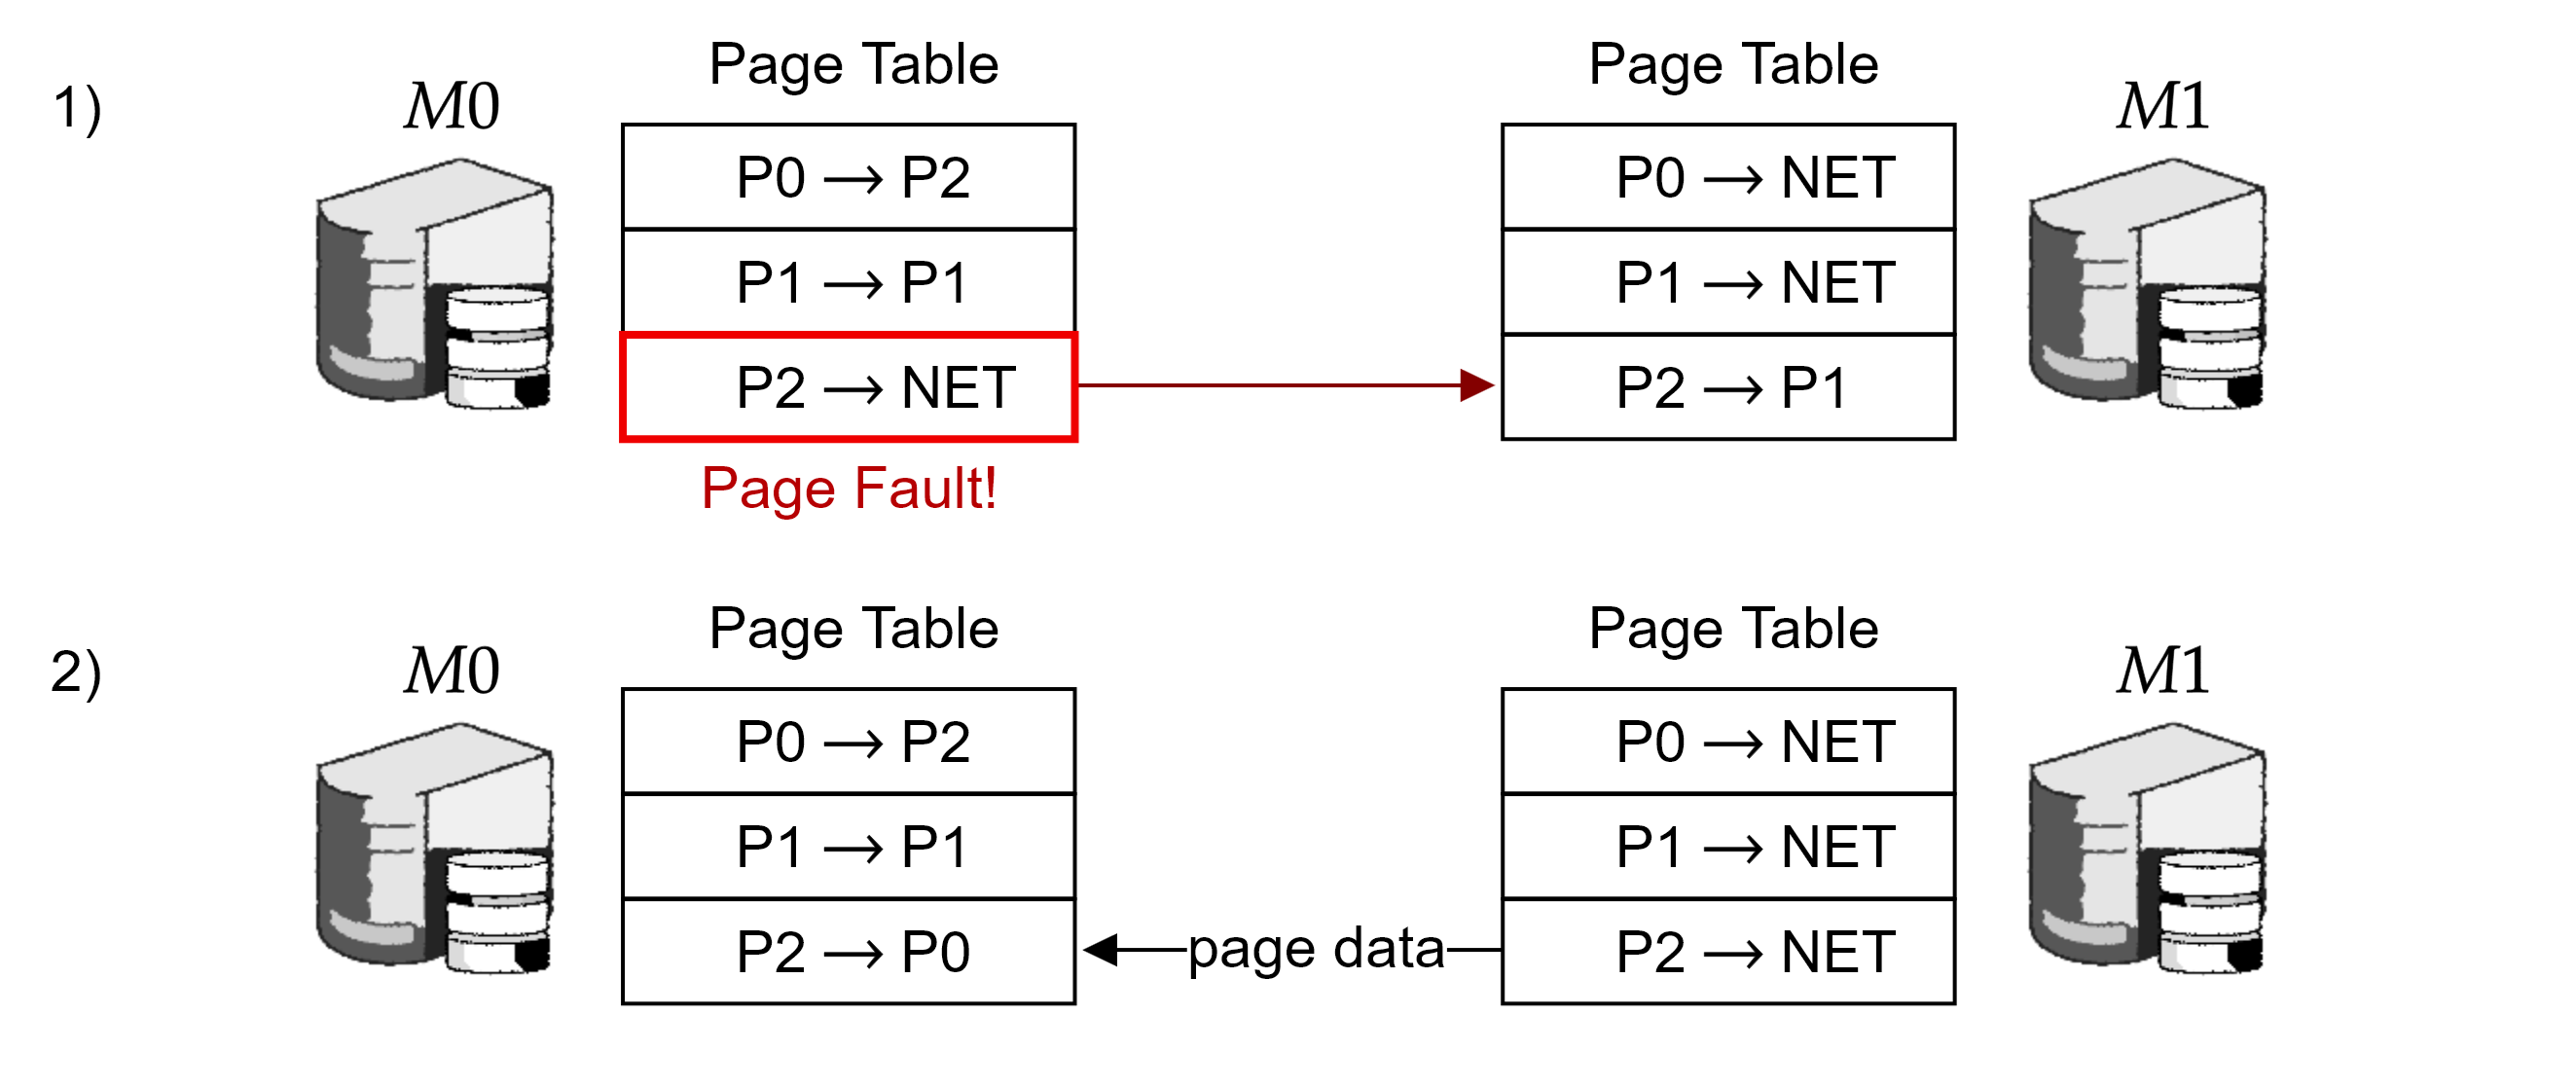
\includegraphics[width=\textwidth]{Sections/shared/share.png}
    \caption{1) System $M_0$ tries to access $P_2$ in virtual memory but incurs a page fault, prompting a request to the DSM system. The DSM resolves that $M_1$ owns the desired page. 
    2) The DSM performs a network swap, sending the actual page data so $M_0$ can load it into physical memory.
    }
    \label{fig:dsm}
\end{figure}

\newpage 

\noindent
Though this is a good start, it's expensive:

\begin{theo}[Sending Pages Over the Network \& False Sharing]

    Pages are often large (4KB), which is expensive to send.
    If two machines $M_0$ and $M_1$ access the same page, but modify different data points (e.g., two different variables),
    the whole page needs to be sent even though the data is not shared. This is called \textbf{false sharing}.
\end{theo}

\noindent
A particular DSM system called \textbf{TreadMarks} solves this problem:
\begin{Def}[TreadMarks -- Page Ownership \& Swap Protocol]

    Given a system of $M_i$ machines, the VAS is evenly divided amongst them.
    When page faults occur, the DSM sends \textbf{diffs} (change history) over the network instead of the entire page.\\

    \noindent
    This allows for all $M_i$ to start with \textbf{RO} (read-only) access on all pages. When $M_j$ wishes to 
    modify a page, $M_j$ notifies all other $M_i$ to invalidate their copies of the page. $M_j$ then gets \textbf{RW} (read-write) access to the page (at most one writeable copy).


    Each write creates a new $V_i$ version of the page ($i$, increases monotonically). Where $V_i$ contains the latest changes, and $V_{i-1}$ a snapshot before the changes.
    
    When $M_i$ page faults, the DSM system requests the page from owner $M_j$, notifying them of the last version $M_i$ saw. The owner $M_j$ locks said page and creates a diff between both $M_i$ and $M_j$'s versions, sending it over the network.
    Both $M_j$ and $M_i$ revert to RO access.\\

    \noindent
    \underline{\textbf{Consistency Model:} Weak consistency} as per lazy-release style of diff sharing.
\end{Def}

\vspace{-1em}
\begin{figure}[h]
    \centering
    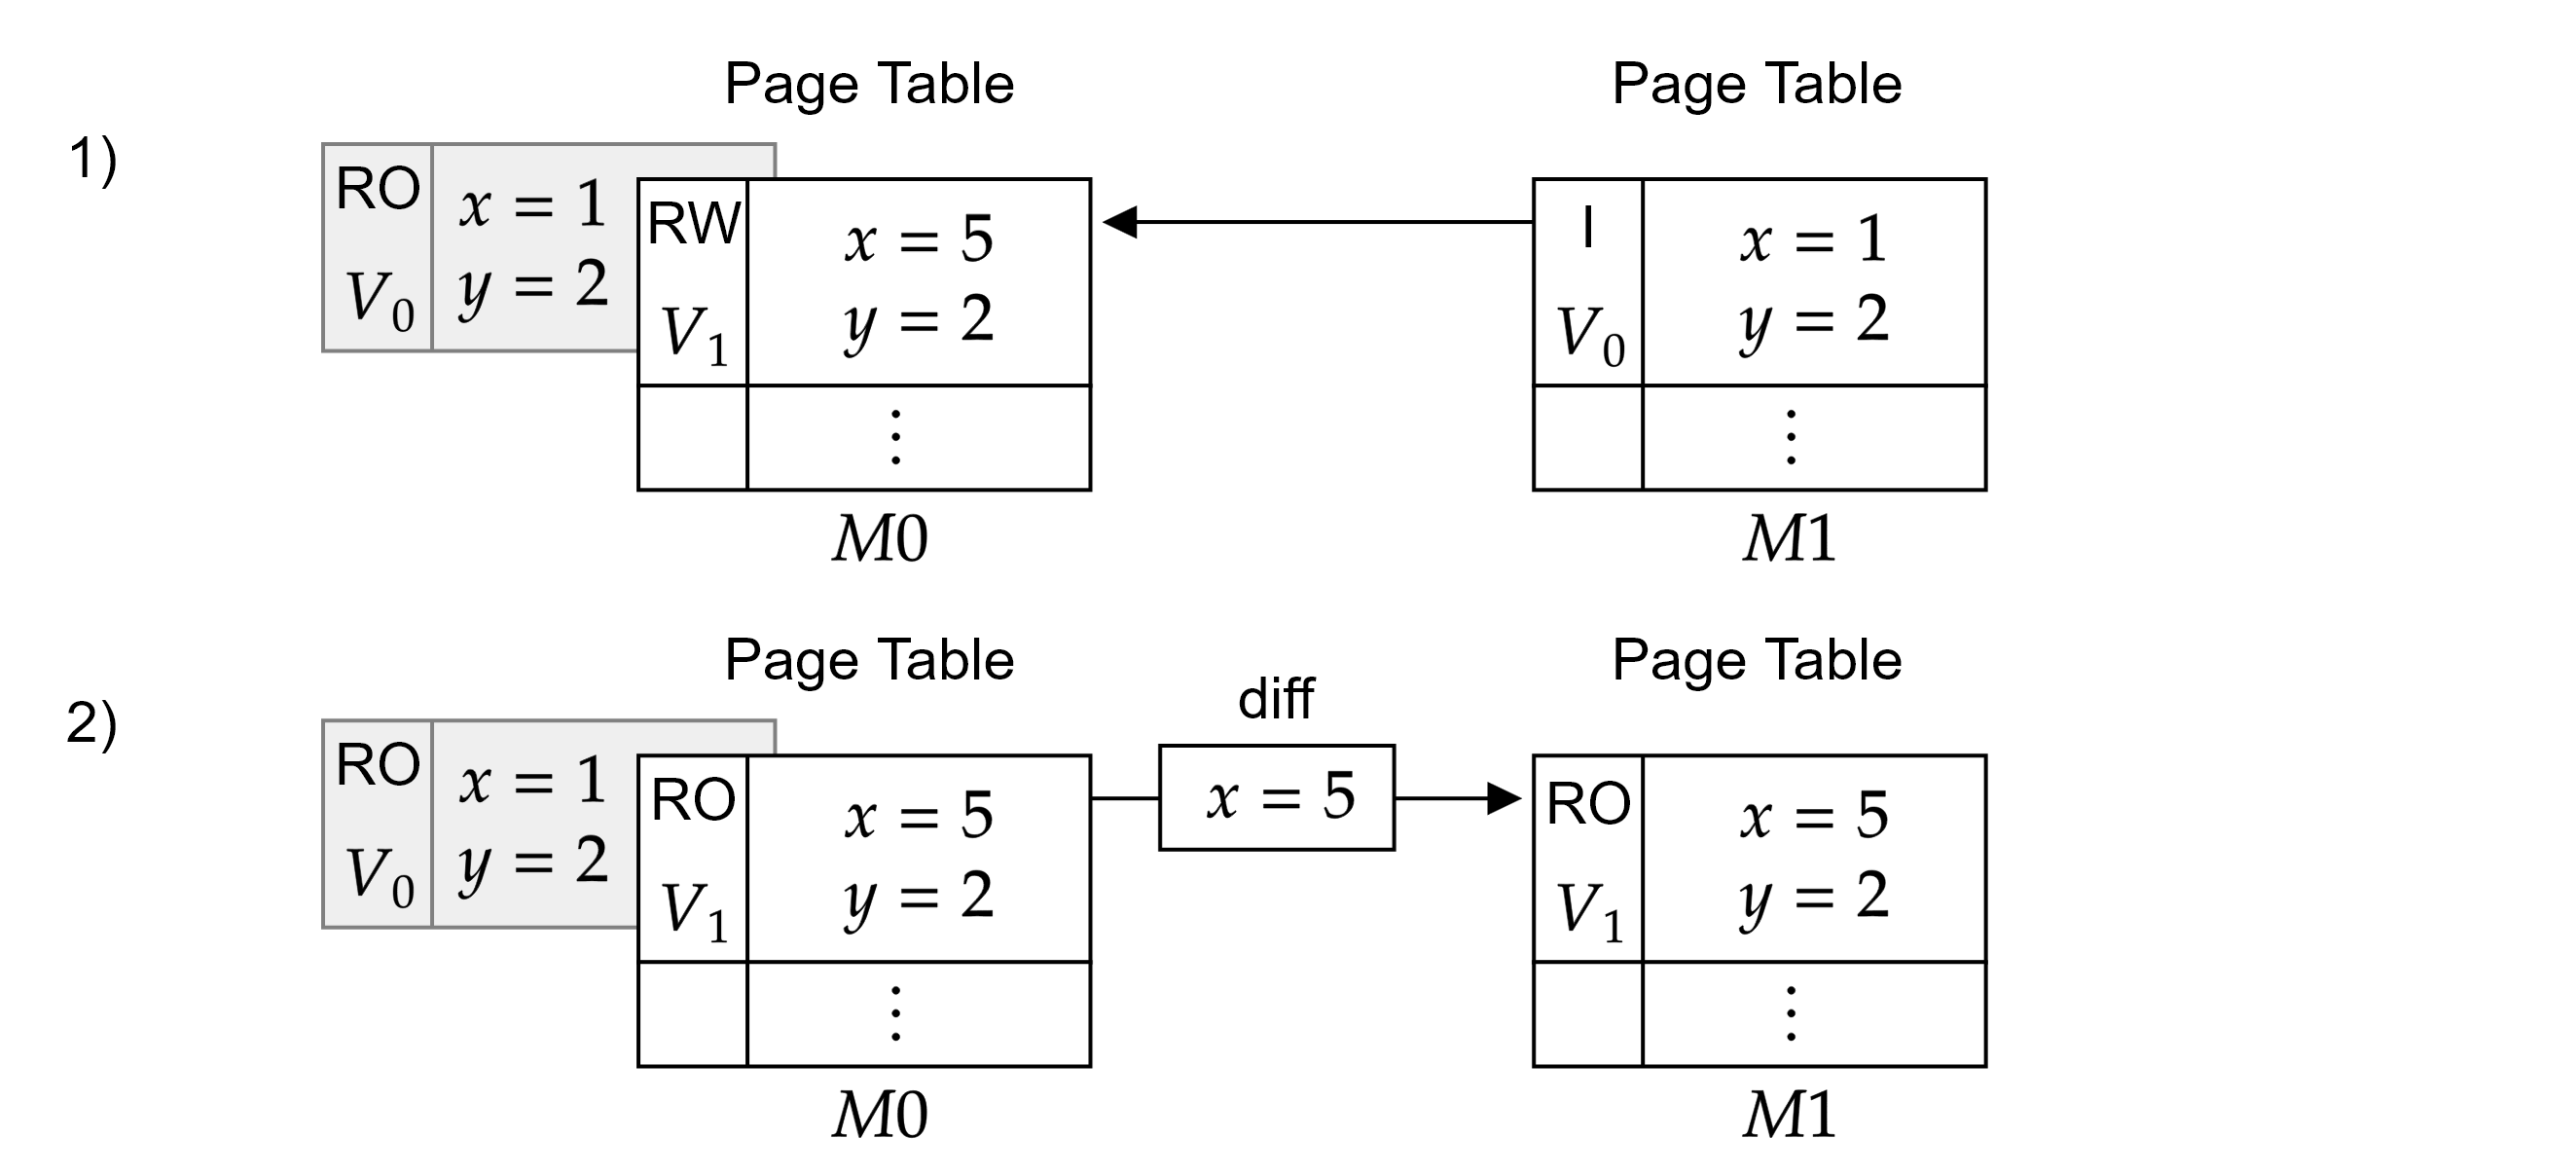
\includegraphics[width=\textwidth]{Sections/shared/tread.png}
    \caption{1) $M1$ requests a page from $M2$. 2) $M2$ sends the diff between $V_0$ and $V_1$ to $M1$.}
    \label{fig:dsm}
\end{figure}

\newpage
\noindent
To ensure that multiple RW access occurs on the same data we send locks over the network.
We briefly discussed these methods in Subsection (\ref{sec:rel}) concerning release consistency.
\begin{Def}[TreadMarks -- Lazy-release]

    TreadMarks utilizes lazy-release consistency to protect against data-races.
    The programmer explicitly locks and unlocks shared data (e.g., mutexes on variables).
    Any page that is dirtied (modified) the dsm generates a diff for. Per lazy-release consistency,
    nodes only require diffs when trying to access data from such pages.
\end{Def}

\noindent
Though this is a good start, it loses the causal relationship between the data.
\begin{Example}[Using Vector Clocks to Capture Causal Consistency]

    Consider the following example at initialization \snippet{x := 0; y := \&x; var z *int}:
    \begin{lstlisting}[language=Go, numbers=none]
1.  // -- Machine M0 -- initial VC = [0,0,0]

    Lock(A)            // acquire lock A
    x = 7              // write to page A
    Unlock(A)          // increments VC[0] -> VC = [1,0,0]; diffA@[1,0,0]

    Lock(B)            // acquire lock B
    y = &x             // write to page B (stores pointer to x)
    Unlock(B)          // increments VC[0] _> VC = [2,0,0]; diffB@[2,0,0]

    \end{lstlisting}

    \begin{lstlisting}[language=Go, numbers=none]
2.  // -- Machine M1 -- initial VC = [0,0,0]

    Lock(B)            // pulls diffs for B newer than [0,0,0]:
                       // gets diffA@[1,0,0] and diffB@[2,0,0]
                       // updates VC to [2,0,0]
    Lock(C)            // acquire lock C
    z = y              // write to page C (stores the pointer y)
    Unlock(C)          // increments VC[1] -> VC = [2,1,0]; diffC@[2,1,0]
    Unlock(B)          // no writes, but would propagate nothing new
    \end{lstlisting}

    \begin{lstlisting}[language=Go, numbers=none]
3.  // -- Machine M2 -- initial VC = [0,0,0]
    
    Lock(C)            // pulls diffs for C newer than [0,0,0]:
                       // diffA@[1,0,0], diffB@[2,0,0], then diffC@[2,1,0]
    print(*z)          // prints 7 as opposed to 0
    Unlock(C)          
    \end{lstlisting}
    \noindent
    Without vector clocks, $M_3$ would have only seen $M_1$'s changes to $C$ (\snippet{z = y}), missing that 
    that $A$ and $B$ were modified before. Therefore $M_3$ would have printed 0 instead of 7.
\end{Example}

\newpage 

\noindent
Hence, we need to employ vector clocks to ensure causality. Let's define it:
\begin{Def}[TreadMarks -- Causal Consistency]

    TreadMarks utilizes vector clocks to ensure causal consistency between page updates.
    Each index of the vector clock corresponds to each machine in the system. Every update monotonically increases $M_i$'s index in the vector clock.\\

    \noindent
    For instance, say there are two machines $M_0$ and $M_1$ with pages $A$ and $B$ respectively, resulting in a vector clock of $[0,0]$.
    If $M_0$ modifies page $A$ then $B$, it would increment its index once for $A$'s diff and then twice for $B$'s diff, yielding $[2,0]$. 
    
    Once $M_1$ reads page $B$, 
    it requests the lock from $M_0$. Along with the lock acquisition comes the diffs for $A$ and $B$.
    Then $M_1$ applies every diff from $M_0$'s vector clock that is greater than its own, resulting in $[2,0]$. Only when $M_1$ modifies page $B$, does its local vector clock increase to $[2,1]$ (while $M_0$'s remains at $[2,0]$).
\end{Def}

\noindent
In summary we need the following components in our RPC API:
\begin{Def}[TreadMarks -- Whole Component Summary]

    We need the following components in our RPC API:

    \begin{itemize}
        \item \textbf{Versioning Control}: Every write to a page creates a new version with a trailing diff.
        \item \textbf{Causal Consistency}: Versioning history for each machine is stored in a vector clock.
        \item \textbf{Locking}: Every page is locked before modification, with a lazy-release system to bypass notifying the entire cluster.

    \end{itemize}

    \noindent
    \underline{\textbf{Consistency Model:} Weak consistency -- Lazy-release + Causal Consistency.}
\end{Def}

\noindent
\textbf{We degraded our consistency} model from strong to weak consistency to save on performance. It is completely 
possible to read stale data in this system; though, it is guaranteed that the data is consistent with the causal relationship of the data.